\documentclass[conference]{IEEEtran}

% -- Core (pdfLaTeX)
\usepackage[utf8]{inputenc}
\usepackage[T1]{fontenc}

% -- Graphics & citations
\usepackage{graphicx}
\usepackage{cite}
\usepackage{url} % for \url in .bib (safe with IEEEtran)

% -- Math
\usepackage{mathtools} % loads amsmath
\usepackage{amssymb}
\usepackage{bm}

% -- Text symbols (optional)
\usepackage{textcomp}

% -- Tables
\usepackage{array}
\usepackage{tabularx}
\usepackage{makecell}
\usepackage{booktabs} % optional (use only if you actually use \toprule etc.)
\graphicspath{{figures/}}

% Column helpers
\newcolumntype{C}[1]{>{\centering\arraybackslash}p{#1}}
\newcolumntype{L}[1]{>{\raggedright\arraybackslash}p{#1}}
\newcolumntype{Y}{>{\raggedright\arraybackslash}X} % for tabularx

% -- Eta helpers
\newcommand{\etav}{\bm{\eta}}
\newcommand{\etavdot}{\dot{\bm{\eta}}}
\newcommand{\etavddot}{\ddot{\bm{\eta}}}

\setlength{\textfloatsep}{8pt}
\setlength{\floatsep}{6pt}
\setlength{\intextsep}{6pt}

\title{Motion Planning and Control of a Differential-Drive Mobile Manipulator}

\author{
\IEEEauthorblockN{Muhammed Elyamani$^{1,2}$, Ali Attyatullah Mohammed AlBeladi$^{1}$, Brahim Brahmi$^{1}$}
\IEEEauthorblockA{$^{1}$King Fahd University of Petroleum \& Minerals (KFUPM)\\
$^{2}$University of Ottawa\\
Emails: g202427600@kfupm.edu.sa, melya038@uottawa.ca, albeladi@kfupm.edu.sa, brahim.brahmi@kfupm.edu.sa}
}




\begin{document}
% near the start (after \begin{document} is fine)
\bstctlcite{BSTcontrol}

\maketitle

\begin{abstract}
This paper presents the modeling, control, and planning of a differential-drive mobile manipulator equipped with a 3-DOF serial arm. A unified motion generation and tracking framework is developed using a structured three-layer architecture consisting of: (i) a motion-planning layer responsible for generating offline/online state-space trajectories in the reduced coordinates  $\etav$; (ii) a kinematic control layer combining Kanayama-based base control with PD joint-velocity control for the manipulator arm; and (iii) a dynamic control layer performing feedback linearization to track the generated references under model nonlinearities. A complete dynamic model is utilized, and robustness is evaluated by injecting disturbances at the torque level. Simulations validate the ability of the proposed architecture to generate feasible trajectories, track them accurately, and maintain performance under disturbances.
\end{abstract}


\begin{IEEEkeywords}
Mobile Manipulator, Motion Planning, Feedback Linearization, Kinematic Control, Differential-Drive Robot, Robust Control.
\end{IEEEkeywords}

\section{Introduction}

\subsection{Background and Motivation}
Mobile manipulators combine a mobile base with a serial robotic arm to achieve both large workspace coverage and dexterous manipulation. This integration enables tasks that are difficult for fixed-base arms, such as in-warehouse handling, service robotics, and field operations. However, coordinating a differential-drive base with an articulated arm remains challenging due to: (i) the base nonholonomic rolling constraint, (ii) strong nonlinear dynamic coupling between base and arm, and (iii) the need to generate reference motions that are not only kinematically feasible but also \emph{dynamically trackable} at the torque level under disturbances and modeling errors. These challenges motivate unified planning--control frameworks in which planning, kinematic coordination, and torque-level tracking are designed consistently.

\subsection{Problem Statement}
This work considers a differential-drive mobile manipulator equipped with a 3-DOF serial arm. Let the full generalized coordinates be
$q=[x_b~y_b~\theta_m~\theta_r~\theta_l~q_1~q_2~q_3]^\top$,
subject to the nonholonomic constraint that prohibits lateral slip.
The objective is to design a modular framework that:
(i) derives a reduced-order dynamic model that embeds the nonholonomic constraint by construction;
(ii) generates smooth, time-parameterized references for the base and arm (offline and optionally online);
(iii) achieves accurate tracking at the torque level using a nonlinear controller; and
(iv) evaluates robustness under additive torque disturbances using tracking and effort/energy metrics.

\subsection{Literature Review}
\noindent\textbf{Nonholonomic control.}
For unicycle and differential-drive vehicles, Kanayama \emph{et al.} proposed a Lyapunov-stable trajectory tracking law widely used for kinematic-level control \cite{kanayamaStableTrackingControl1990a}. Fundamental results on modeling and stabilization limitations for nonholonomic mechanical systems were established in \cite{blochControlStabilizationNonholonomic1992}.

\noindent\textbf{Coordinated mobile manipulation.}
Early work emphasized vehicle--arm coordination and task execution on mobile platforms \cite{khatibMobileManipulatorsExpanding1998}. Yamamoto and Yun studied coordination strategies and quantified how base--arm dynamic interaction affects tracking performance \cite{yamamotoCoordinatingLocomotionManipulation1994,yamamotoEffectDynamicInteraction1996}. Seraji proposed a unified formulation that exploits base mobility and redundancy during motion generation \cite{serajiUnifiedApproachMotion1998}. For wheeled mobile robots, dynamic feedback linearization was shown to provide precise tracking and regulation capabilities \cite{orioloWMRControlDynamic2002}.

\noindent\textbf{Integrated planning--control.}
Recent approaches increasingly couple motion generation and control through whole-body constraints and reactive behaviors \cite{havilandHolisticApproachReactive2022}, task-level planning for pickup/transport while the base moves \cite{thakarManipulatorMotionPlanning2022}, and perceptive MPC that incorporates exteroceptive and haptic feedback for continuous mobile manipulation \cite{pankertPerceptiveModelPredictive2020}. Coordinated planning/control frameworks have also been extended to include manipulability optimization and hybrid motion/force tracking for more complex platforms \cite{zhangCoordinatedPlanningControl2025a}.

\noindent\textbf{Gap and motivation.}
While existing methods address important aspects of mobile manipulation, a recurring practical gap is ensuring that the planned references remain \emph{dynamically trackable} under a constraint-consistent reduced model and that robustness can be evaluated in a repeatable way at the torque level.

\subsection{Contribution}
This paper presents a baseline, reproducible planning and control stack for a differential-drive mobile manipulator. The main contributions are:
\begin{itemize}
  \item \textbf{Constraint-consistent reduced dynamics in independent coordinates.}
  We embed the rolling constraint through a null-space velocity parametrization, yielding a compact reduced model in
  $\etav=[\theta_r~\theta_l~q_1~q_2~q_3]^\top$ suitable for torque-level control.
  
  \item \textbf{Three-layer architecture with a clean reference interface.}
  We implement a modular pipeline (planner $\rightarrow$ kinematics $\rightarrow$ dynamics) that supports offline references and an optional online planner, and produces smooth $(\etav_d,\dot{\etav}_d,\ddot{\etav}_d)$ trajectories consistent with the reduced model.
  
  \item \textbf{Torque-level tracking via feedback linearization and robustness evaluation.}
  A reduced-coordinate feedback linearization controller enforces linear error dynamics, and robustness is assessed by injecting additive torque disturbances (bias/sinusoidal/Gaussian) while reporting tracking error, control effort, and energy
  $E=\int_{0}^{T_f}\tau^\top \dot{\etav}\,dt$.
\end{itemize}


\section{System Modeling}
\label{sec:system_modeling}

This section derives a constraint-consistent dynamic model of the differential--drive mobile manipulator. The base is subject to a rolling nonholonomic constraint, and the overall system exhibits coupled nonlinear dynamics due to the interaction between the mobile platform and the serial arm. To obtain equations suitable for torque-level control design, the constraint is embedded directly through a reduced velocity parametrization. The resulting reduced-order model evolves in independent coordinates and satisfies feasibility by construction.

% -----------------------------
\subsection{Robot Geometry and Coordinate Frames}
\label{subsec:frames}

Fig.~\ref{fig:Side_view_X_Z_plane} shows a side view of the mobile manipulator in the $X$--$Z$ plane, highlighting the base and the 3-DOF arm geometry used in modeling.

\begin{figure}[t]
    \centering
    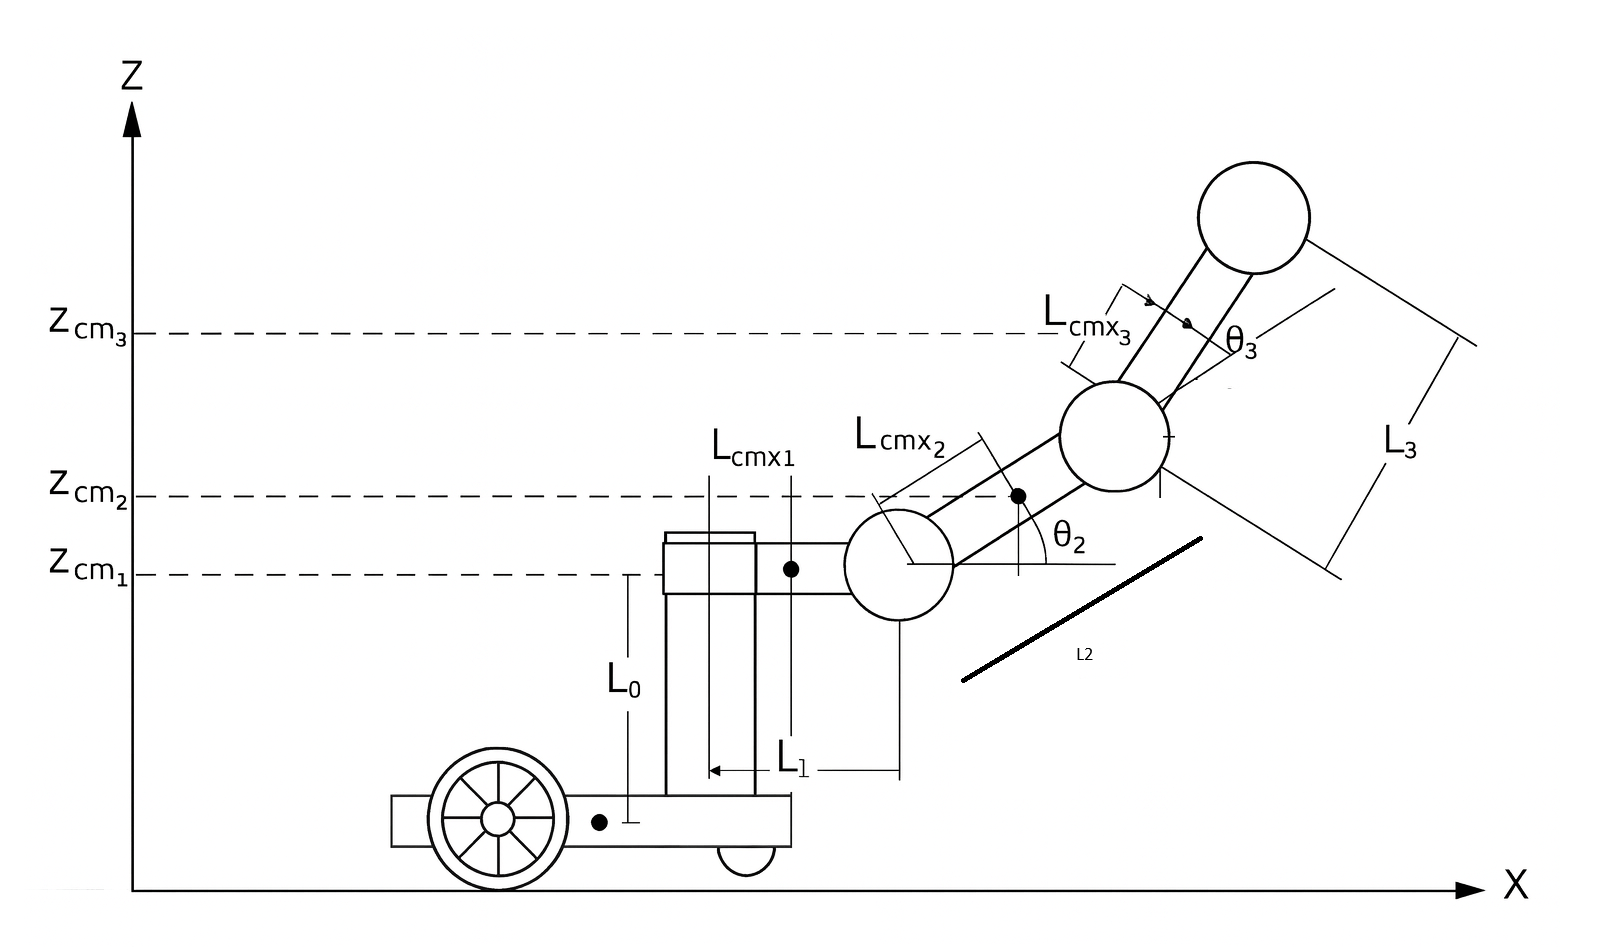
\includegraphics[width=\columnwidth]{figures/Side_view_X_Z_plane}
    \caption{Side view of the mobile manipulator in the $X$--$Z$ plane.}
    \label{fig:Side_view_X_Z_plane}
\end{figure}

% -----------------------------
\subsection{Generalized Coordinates and Actuation}
\label{subsec:q_tau}

The configuration is described by
\begin{equation}
q =
\begin{bmatrix}
x_b & y_b & \theta_m & \theta_r & \theta_l & q_1 & q_2 & q_3
\end{bmatrix}^{\!\top}\in \mathbb{R}^{8},
\label{eq:q_def}
\end{equation}
where $(x_b,y_b,\theta_m)$ denote the planar pose of the \emph{mounting frame} rigidly attached to the base, $\theta_r$ and $\theta_l$ are the right/left wheel angles, and $q_1,q_2,q_3$ are the arm joint coordinates.

The actuator torque vector is
\begin{equation}
\tau =
\begin{bmatrix}
\tau_r & \tau_l & \tau_1 & \tau_2 & \tau_3
\end{bmatrix}^{\!\top}\in\mathbb{R}^{5},
\label{eq:tau_def}
\end{equation}
corresponding to the two wheel motors and three arm joints. Let $B(q)\in\mathbb{R}^{8\times 5}$ denote the actuation distribution matrix such that generalized forces are $B(q)\tau$.

% -----------------------------
\subsection{Lagrange--d'Alembert Dynamics with Nonholonomic Constraint}
\label{subsec:constrained_dyn}

Let $\mathcal{L}(q,\dot q)=T(q,\dot q)-U(q)$ be the Lagrangian. Using the Lagrange--d'Alembert principle with Pfaffian nonholonomic constraints, the constrained dynamics can be written as
\begin{equation}
M(q)\ddot q + C(q,\dot q)\dot q + D(q)\dot q + G(q)
=
B(q)\tau + A^\top(q)\lambda,
\label{eq:full_constrained_dyn}
\end{equation}
where $M(q)$ is the inertia matrix, $C(q,\dot q)\dot q$ collects Coriolis/centrifugal effects, $D(q)\dot q$ represents viscous dissipation, $G(q)$ is the gravity vector, $A(q)\dot q = 0$ encodes the nonholonomic constraints, and $\lambda$ are Lagrange multipliers (constraint forces) \cite{blochControlStabilizationNonholonomic1992}.

% -----------------------------
\subsection{Nonholonomic Rolling Constraint}
\label{subsec:nh_constraint}

For a differential-drive base, lateral slip at the mounting frame is prohibited. In world coordinates,
\begin{equation}
\dot{x}_b \sin\theta_m - \dot{y}_b \cos\theta_m = 0,
\label{eq:nonholonomic}
\end{equation}
which is compactly written as $A(q)\dot q = 0$ with $A(q)\in\mathbb{R}^{1\times 8}$.

% -----------------------------
\subsection{Independent Coordinates and Constraint-Consistent Velocity Mapping}
\label{subsec:eta_R}

We define the independent coordinates as the actuated generalized coordinates
\begin{equation}
\etav =
\begin{bmatrix}
\theta_r & \theta_l & q_1 & q_2 & q_3
\end{bmatrix}^{\!\top}\in\mathbb{R}^{5},
\label{eq:eta_def}
\end{equation}
with velocities $\dot{\etav}$ and accelerations $\ddot{\etav}$.

To enforce the rolling constraint by construction, the full generalized velocity is parametrized as
\begin{equation}
\dot q = R(q)\dot{\etav},
\label{eq:qdot_R}
\end{equation}
where $R(q)\in\mathbb{R}^{8\times 5}$ is chosen such that
\begin{equation}
A(q)R(q)=0.
\label{eq:AR0}
\end{equation}
This guarantees that any motion generated through \eqref{eq:qdot_R} is admissible and that constraint forces vanish when projecting onto the null-space of $A(q)$.

% -----------------------------
\subsection{Wheel-Rate to Base-Twist Mapping at the Mounting Frame}
\label{subsec:Rbase}

Following the coupled modeling convention in \cite{prada-jimenezCoupledDynamicModel2019a}, the differential-drive kinematics at the mounting frame can be expressed as a linear mapping from wheel rates to base twist components:
\begin{equation}
\begin{bmatrix}
\dot{x}_b\\
\dot{y}_b\\
\dot{\theta}_m\\
\dot{\theta}_r\\
\dot{\theta}_l
\end{bmatrix}
=
R_{\mathrm{base}}(\theta_m)
\begin{bmatrix}
\dot{\theta}_r\\
\dot{\theta}_l
\end{bmatrix},
\label{eq:base_map}
\end{equation}
where $r$ is the wheel radius, $2L$ is the axle length, and $d$ is the longitudinal offset between the axle midpoint and the mounting frame.

\begin{equation}
\resizebox{\columnwidth}{!}{$
R_{\mathrm{base}}(\theta_m)=
\begin{bmatrix}
\frac{r}{2L}(L\cos\theta_m-d\sin\theta_m) &
\frac{r}{2L}(L\cos\theta_m+d\sin\theta_m)\\
\frac{r}{2L}(L\sin\theta_m+d\cos\theta_m) &
\frac{r}{2L}(L\sin\theta_m-d\cos\theta_m)\\
\frac{r}{2L} & -\frac{r}{2L}\\
1 & 0\\
0 & 1
\end{bmatrix}
$}
\label{eq:Rbase}
\end{equation}

The complete mapping $R(q)$ is formed by appending the arm joint rates:
\begin{equation}
R(q)=
\begin{bmatrix}
R_{\mathrm{base}}(\theta_m) & 0_{5\times 3}\\
0_{3\times 2} & I_3
\end{bmatrix}.
\label{eq:R_full}
\end{equation}

% -----------------------------
\subsection{Reduced-Order Dynamics in Independent Coordinates}
\label{subsec:reduced_dyn}

Differentiating \eqref{eq:qdot_R} yields
\begin{equation}
\ddot q = R(q)\ddot{\etav} + \dot R(q,\dot q)\dot{\etav}.
\label{eq:qddot_R}
\end{equation}
Substituting \eqref{eq:qdot_R}--\eqref{eq:qddot_R} into \eqref{eq:full_constrained_dyn} and premultiplying by $R^\top(q)$ eliminates the constraint forces because
$R^\top A^\top = (AR)^\top = 0^\top$. The reduced model becomes
\begin{equation}
M_1(q)\ddot{\etav}
+
C_1(q,\dot q)\dot{\etav}
+
D_1(q)\dot{\etav}
+
G_1(q)
=
B_1(q)\tau,
\label{eq:reduced_dyn}
\end{equation}
with
\begin{align}
M_1(q) &= R^\top(q)M(q)R(q),\\
C_1(q,\dot q) &= R^\top(q)\!\left[M(q)\dot R(q,\dot q)+C(q,\dot q)R(q)\right],\\
D_1(q) &= R^\top(q)D(q)R(q),\\
G_1(q) &= R^\top(q)G(q),\\
B_1(q) &= R^\top(q)B(q).
\end{align}

Equation \eqref{eq:reduced_dyn} preserves base--arm coupling while guaranteeing feasibility with respect to the nonholonomic constraint. It is therefore convenient for torque-level nonlinear control design (e.g., feedback linearization), since it evolves directly in $\etav$ and avoids explicit computation of $\lambda$ \cite{prada-jimenezCoupledDynamicModel2019a}.

% -----------------------------
\subsection{Remark on Simulation Consistency}
\label{subsec:sim_consistency}

In simulation, the reduced model is integrated using the state
$X=[q^\top~\dot{\etav}^\top]^\top$. Whenever quantities depending on $\dot q$
are required (e.g., in $C_1(q,\dot q)$ or $\dot R$), the full generalized
velocity is reconstructed using \eqref{eq:qdot_R}. This preserves constraint
consistency throughout the closed-loop simulation.

\section{Three-Layer Control Architecture}
\label{sec:three_layer_arch}

This section presents the proposed hierarchical control framework for the
differential--drive mobile manipulator. The architecture is organized into
three layers: (i) a motion--planning layer that generates smooth reference
trajectories; (ii) a kinematic coordination layer that converts pose/joint
references into admissible velocity commands while enforcing the base
nonholonomic constraint; and (iii) a torque--level dynamic tracking layer that
compensates for nonlinear coupled dynamics in the reduced independent
coordinates $\etav$. The separation improves modularity and allows each layer
to be designed and tested independently.

\subsection{Signal Flow and Interfaces}
\label{subsec:signals_interfaces}

Let $\etav=[\theta_r~\theta_l~q_1~q_2~q_3]^\top$ denote the independent
coordinates and let $(\etav_d,\dot{\etav}_d,\ddot{\etav}_d)$ denote their
references. At each time $t$, the layers exchange the following signals:
\begin{itemize}
  \item \textbf{Layer~3 $\rightarrow$ Layer~2:} base pose/twist references
  $(x_r,y_r,\theta_r,v_r,\omega_r)$ at the mounting frame $B$, and joint
  references $(q_d,\dot q_d,\ddot q_d)$.
  \item \textbf{Layer~2 $\rightarrow$ Layer~1:} commanded independent-velocity
  reference $\dot{\etav}_d$ (and optionally a smoothed $\ddot{\etav}_d$), and
  measured $(\etav,\dot{\etav})$ from the plant/simulator.
  \item \textbf{Layer~1 output:} actuator torques $\tau\in\mathbb{R}^5$ applied
  to wheels and arm joints.
\end{itemize}

\subsection{Layer 3: Motion Planning}
\label{subsec:layer3_planning}

Layer~3 generates smooth time-parameterized trajectories for the base and the
arm over a finite horizon $T_f$. The objective is to provide references with
continuous position, velocity, and acceleration, suitable for torque-level
tracking.

\subsubsection{Planning frames}

Geometric planning is performed in the axle-center frame $M$ (wheel midpoint),
while tracking and logging are performed in the mounting frame $B$ attached to
the manipulator base. The rigid body offset from $M$ to $B$ expressed in the
body frame is ${}^{M}\!p_{MB}=[d_x~d_y]^\top$ (constant). Start/goal poses are
converted once so that both $p_0^M,p_f^M$ and $p_0^B,p_f^B$ are consistent.

\subsubsection{Base reference generation (R--T--R with quintic timing)}

Given start and goal poses in frame $M$,
$p_0^M=(x_{M0},y_{M0},\theta_0)$ and $p_f^M=(x_{Mf},y_{Mf},\theta_f)$, define
\begin{equation}
d = \sqrt{(x_{Mf}-x_{M0})^2 + (y_{Mf}-y_{M0})^2},
\end{equation}
\begin{equation}
\theta_{\mathrm{line}} =
\begin{cases}
\theta_0, & d \approx 0,\\
\mathrm{atan2}(y_{Mf}-y_{M0},\,x_{Mf}-x_{M0}), & \text{otherwise}.
\end{cases}
\end{equation}
The motion is decomposed into rotate--translate--rotate segments with
\begin{equation}
\Delta\theta_1 = \mathrm{wrap}(\theta_{\mathrm{line}}-\theta_0),\qquad
\Delta\theta_2 = \mathrm{wrap}(\theta_f-\theta_{\mathrm{line}}),
\end{equation}
and each segment is time-scaled using the quintic
\begin{equation}
\sigma(\tau)=10\tau^3-15\tau^4+6\tau^5,\qquad \tau\in[0,1],
\end{equation}
to ensure $C^2$ continuity (zero endpoint velocity and acceleration). The
result is an analytical trajectory for $(x_M(t),y_M(t),\theta(t))$ and their
derivatives.

\subsubsection{Mapping from center frame $M$ to mounting frame $B$}

The reference is mapped to the mounting point via rigid-body kinematics:
\begin{equation}
\begin{bmatrix}x_B\\y_B\end{bmatrix}
=
\begin{bmatrix}x_M\\y_M\end{bmatrix}
+
R(\theta)\begin{bmatrix}d_x\\d_y\end{bmatrix},
\qquad \theta_B=\theta,
\end{equation}
where $R(\theta)$ is the planar rotation matrix. Differentiation provides
consistent $\dot x_B,\dot y_B,\ddot x_B,\ddot y_B$ including tangential and
centripetal terms due to rotation.

The body-frame reference twist at $B$ is computed as
\begin{equation}
v_r = \cos\theta\,\dot{x}_B + \sin\theta\,\dot{y}_B,\qquad
\omega_r = \dot{\theta}.
\label{eq:vr_omega_r}
\end{equation}

\subsubsection{Arm joint reference generation}

Each joint is planned in joint space using a fifth-order polynomial
$q_i(t)=\sum_{k=0}^{5} a_{ik} t^k$ satisfying boundary conditions on
$q_i,\dot q_i,\ddot q_i$ at $t=0$ and $t=T_f$. This yields smooth
$(q_d,\dot q_d,\ddot q_d)$ with zero endpoint transients.

\subsection{Layer 2: Kinematic Coordination}
\label{subsec:layer_kinematics}

Layer~2 converts the planned references into admissible velocity commands for
the nonholonomic base and the arm joints. This layer does not require dynamic
parameters, and provides a robust interface between planning and torque-level
tracking.

\subsubsection{Base kinematic tracking (Kanayama-type law)}

The base is modeled as a unicycle:
\begin{equation}
\dot x = v\cos\theta,\qquad
\dot y = v\sin\theta,\qquad
\dot\theta = \omega.
\end{equation}
Let $(x_r,y_r,\theta_r)$ and $(v_r,\omega_r)$ be the reference pose and twist at
the mounting frame $B$. Define position error in world coordinates
$\Delta p=[x_r-x~~y_r-y]^\top$ and transform it into the robot frame:
\begin{equation}
\begin{bmatrix}x_e\\y_e\end{bmatrix}
=
\begin{bmatrix}
\cos\theta & \sin\theta\\
-\sin\theta & \cos\theta
\end{bmatrix}
\Delta p.
\end{equation}
Define heading error
\begin{equation}
\theta_e=\mathrm{atan2}\!\big(\sin(\theta_r-\theta),\cos(\theta_r-\theta)\big).
\end{equation}
The commanded velocities are
\begin{equation}
v_c = v_r\cos\theta_e + K_x x_e,
\label{eq:kanayama_v}
\end{equation}
\begin{equation}
\omega_c = \omega_r + v_r\big(K_y y_e + K_\theta \sin\theta_e\big),
\label{eq:kanayama_omega}
\end{equation}
with positive gains $K_x,K_y,K_\theta$. Optional saturation on $v_c,\omega_c$
can be applied to respect actuator limits.

\subsubsection{Arm joint velocity control (PD with feedforward)}

Let $(q,\dot q)$ be measured arm states and $(q_d,\dot q_d)$ the desired
trajectories. Define errors
\begin{equation}
e_q=q_d-q,\qquad e_{\dot q}=\dot q_d-\dot q.
\end{equation}
A velocity command is computed as
\begin{equation}
\dot q_c=\dot q_d + K_p^{(a)} e_q + K_d^{(a)} e_{\dot q},
\label{eq:arm_pd}
\end{equation}
where $K_p^{(a)},K_d^{(a)}\succ0$ are diagonal or full gain matrices.

\subsubsection{Mapping to independent coordinate references}

The commanded base velocities $(v_c,\omega_c)$ are converted to wheel-rate
references using differential-drive kinematics:
\begin{equation}
\dot{\theta}_{r,d}=\frac{1}{r}\big(v_c+L\omega_c\big),\qquad
\dot{\theta}_{l,d}=\frac{1}{r}\big(v_c-L\omega_c\big),
\label{eq:wheel_rates_from_vw}
\end{equation}
with wheel radius $r$ and half axle length $L$. The complete independent
velocity reference becomes
\begin{equation}
\dot{\etav}_d=
\begin{bmatrix}
\dot{\theta}_{r,d} & \dot{\theta}_{l,d} & \dot q_c^\top
\end{bmatrix}^{\!\top}.
\label{eq:eta_dot_ref}
\end{equation}
When an analytical $\ddot{\etav}_d$ is unavailable, it is obtained by filtering
or finite-difference differentiation on a reference grid.

\subsection{Layer 1: Dynamic Tracking Control}
\label{subsec:layer_dynamics}

Layer~1 operates at the torque level and enforces accurate tracking of the
independent-coordinate references while compensating for nonlinear coupled
dynamics.

\subsubsection{Reduced dynamic model}

Using the reduced formulation in Section~\ref{sec:system_modeling}, the coupled
dynamics in $\etav$ are
\begin{equation}
M_1(q)\ddot{\etav}
+
\big(C_1(q,\dot q)+D_\eta\big)\dot{\etav}
+
G_1(q)
=
B_1(q)\tau,
\label{eq:reduced_dyn_layer1}
\end{equation}
where $D_\eta\succ0$ is an added viscous damping matrix. The full generalized
velocity required by $C_1(q,\dot q)$ is reconstructed via
$\dot q = R(q)\dot{\etav}$.

\subsubsection{Tracking error dynamics and virtual control}

Define tracking errors
\begin{equation}
e=\etav-\etav_d,\qquad \dot e=\dot{\etav}-\dot{\etav}_d.
\end{equation}
Choose a virtual acceleration input
\begin{equation}
v=\ddot{\etav}_d - K_d \dot e - K_p e,
\label{eq:virtual_v}
\end{equation}
with $K_p,K_d\succ0$, yielding the desired linear error dynamics
\begin{equation}
\ddot e + K_d \dot e + K_p e = 0.
\label{eq:err_dyn}
\end{equation}

\subsubsection{Feedback linearization torque law}

From \eqref{eq:reduced_dyn_layer1}, the torque command is selected as
\begin{equation}
\tau
=
B_1^{-1}(q)
\Big(
M_1(q)v
+
\big(C_1(q,\dot q)+D_\eta\big)\dot{\etav}
+
G_1(q)
\Big),
\label{eq:tau_fbl}
\end{equation}
which cancels the nonlinear dynamics (up to modeling error) and enforces
\eqref{eq:err_dyn}.

\subsubsection{Lyapunov stability}

Consider the Lyapunov function
\begin{equation}
V(e,\dot e)=\frac{1}{2}\dot e^\top \dot e + \frac{1}{2} e^\top K_p e.
\end{equation}
Using \eqref{eq:err_dyn},
\begin{equation}
\dot V = -\dot e^\top K_d \dot e \le 0,
\end{equation}
which implies asymptotic convergence to $e=\dot e=0$ under exact cancellation
and standard smoothness assumptions. In practice, $D_\eta$ and the gains
$(K_p,K_d)$ tune the tracking/effort trade-off and improve robustness to
unmodeled effects.

\subsubsection{Disturbance injection for robustness evaluation}

Robustness is evaluated by applying additive torque disturbances:
\begin{equation}
\tau(t)=\tau_{\mathrm{cmd}}(t)+\tau_d(t),
\label{eq:tau_disturbed}
\end{equation}
where $\tau_{\mathrm{cmd}}$ is given by \eqref{eq:tau_fbl}. Disturbances are
chosen as bias, sinusoidal, or Gaussian processes to emulate constant load,
periodic perturbations, and stochastic actuator/interaction effects.

\subsection{Effort and Energy Metrics}
\label{subsec:effort_energy}

The instantaneous mechanical power in the reduced coordinates is
\begin{equation}
P(t)=\tau^\top(t)\dot{\etav}(t),
\end{equation}
and the cumulative control energy is
\begin{equation}
E(t)=\int_{0}^{t} P(\sigma)\,d\sigma,
\end{equation}
reported at $t=T_f$ alongside RMS/max tracking errors for quantitative
comparison across disturbance conditions.

% =========================================================
% =========================================================
% =========================================================
% =========================================================
% =========================================================
% =========================================================
% =========================================================
\section{Simulation Setup}
\label{sec:sim_setup}
% =========================================================
This section summarizes the parameters required to reproduce the simulation results:
(i) robot physical parameters, (ii) scenario boundary conditions, (iii) controller gains and
their tuning rationale, and (iv) numerical integration, robustness disturbances, and metrics.
Physical and motion parameters are specified explicitly in Table~\ref{tab:phys_params} and
Table~\ref{tab:scenario_bc}. These values define the exact robot model and task boundary
conditions used to generate the results reported in Section~\ref{sec:sim_results}.


% ---------------------------------------------------------
\subsection{Robot Physical Parameters}
% ---------------------------------------------------------
Table~\ref{tab:phys_params} lists the physical parameters (SI units) used by the dynamic model.

\begin{table}[t]
\centering
\caption{Physical parameters used in simulation (SI units).}
\label{tab:phys_params}
\scriptsize
\setlength{\tabcolsep}{3.2pt} % <-- key to avoid overlap
\renewcommand{\arraystretch}{1.05}
\resizebox{\columnwidth}{!}{%
\begin{tabular}{|c|c|c||c|c|c|}
\hline
\textbf{Symbol} & \textbf{Value} & \textbf{Units} &
\textbf{Symbol} & \textbf{Value} & \textbf{Units} \\
\hline
$L$        & 0.250  & m     & $L_{\mathrm{cm}x_m}$ & 0.2268 & m \\
$d$        & 0.270  & m     & $L_{\mathrm{cm}x_1}$ & 0.1670 & m \\
$r$        & 0.075  & m     & $L_{\mathrm{cm}x_2}$ & 0.2460 & m \\
$L_0$      & 0.325  & m     & $L_{\mathrm{cm}x_3}$ & 0.1500 & m \\
$L_1$      & 0.200  & m     & $m_1$ & 3.293  & kg \\
$L_2$      & 0.300  & m     & $m_2$ & 3.436  & kg \\
$L_3$      & 0.300  & m     & $m_3$ & 1.229  & kg \\
$m_m$      & 19.2372& kg    & $m_w$ & 0.901  & kg \\
$g$        & 9.81   & m/s$^2$ & $I_m$ & 0.7004 & kg$\cdot$m$^2$ \\
$I_{yyw}$  & 0.0015 & kg$\cdot$m$^2$ & $I_{zzw}$ & 0.0030 & kg$\cdot$m$^2$ \\
$I_{xx1}$  & 0.0053 & kg$\cdot$m$^2$ & $I_{yy1}$ & 0.0221 & kg$\cdot$m$^2$ \\
$I_{zz1}$  & 0.0230 & kg$\cdot$m$^2$ & $I_{xx2}$ & 0.0054 & kg$\cdot$m$^2$ \\
$I_{yy2}$  & 0.0457 & kg$\cdot$m$^2$ & $I_{zz2}$ & 0.0461 & kg$\cdot$m$^2$ \\
$I_{xx3}$  & 0.0017 & kg$\cdot$m$^2$ & $I_{yy3}$ & 0.0242 & kg$\cdot$m$^2$ \\
$I_{zz3}$  & 0.0255 & kg$\cdot$m$^2$ &  &  &  \\
\hline
\end{tabular}%
}
\end{table}

% ---------------------------------------------------------
\subsection{Scenario Boundary Conditions}
% ---------------------------------------------------------
The base trajectory is planned in $\mathrm{SE}(2)$ over a horizon $T_f$ from the start
to goal pose in the mount frame. The arm reference is generated using quintic polynomials with
zero endpoint velocities and accelerations. Boundary conditions are listed in Table~\ref{tab:scenario_bc}.

\begin{table}[t]
\centering
\caption{Scenario boundary conditions used in simulation.}
\label{tab:scenario_bc}
\scriptsize
\setlength{\tabcolsep}{4pt}
\renewcommand{\arraystretch}{1.10}
\resizebox{\columnwidth}{!}{%
\begin{tabular}{|l|c|c|}
\hline
\textbf{Quantity} & \textbf{Symbol} & \textbf{Value} \\
\hline
Planning horizon & $T_f$ & 10 s \\
Base start pose (mount frame) & $(x_0,y_0,\theta_0)$ & $(0,\,0,\,0)$ \\
Base goal pose (mount frame)  & $(x_f,y_f,\theta_f)$ & $(2,\,2,\,\pi/2)$ \\
Arm joint start & $q_0$ & $[0,\,-0.3,\,0.5]^{\top}$ rad \\
Arm joint goal  & $q_f$ & $[2.0,\,0.2,\,-0.4]^{\top}$ rad \\
Endpoint joint velocities & $\dot q(0)=\dot q(T_f)$ & 0 \\
Endpoint joint accelerations & $\ddot q(0)=\ddot q(T_f)$ & 0 \\
Nominal speeds (time allocation) & $(v_{\mathrm{nom}},\omega_{\mathrm{nom}})$ & $(5~\mathrm{m/s},\,5~\mathrm{rad/s})$ \\
\hline
\end{tabular}%
}
\end{table}

% ---------------------------------------------------------
\subsection{Controller Gains and Tuning Rationale}
% ---------------------------------------------------------
Table~\ref{tab:gains} reports gains used in the kinematic and dynamic layers: Kanayama base tracking,
velocity-level PD for the arm, and torque-level feedback-linearization tracking in reduced coordinates $\bm{\eta}$.

\begin{table}[t]
\centering
\caption{Gains used in the kinematic and dynamic control layers.}
\label{tab:gains}
\scriptsize
\setlength{\tabcolsep}{3.2pt}
\renewcommand{\arraystretch}{1.10}
\resizebox{\columnwidth}{!}{%
\begin{tabular}{|l|c|c|}
\hline
\textbf{Controller} & \textbf{Parameter} & \textbf{Value} \\
\hline
Base kinematic tracking (Kanayama) & $(K_x,\,K_y,\,K_\theta)$ & $(5.0,\,5.0,\,2.0)$ \\
Arm kinematic control (velocity PD) & $K_p$ & $\mathrm{diag}(2,2,2)$ \\
Arm kinematic control (velocity PD) & $K_d$ & $\mathrm{diag}(1,1,1)$ \\
Dynamic tracking (error shaping in $\bm{\eta}$) & $\zeta$ & 1.0 \\
Dynamic tracking (wheel DOFs) & $\omega_{n,\mathrm{base}}$ & 2.0 rad/s \\
Dynamic tracking (arm DOFs) & $\omega_{n,\mathrm{arm}}$ & 1.5 rad/s \\
Resulting $K_p$ in $\bm{\eta}$ & $K_p$ & $\mathrm{diag}(4,4,2.25,2.25,2.25)$ \\
Resulting $K_d$ in $\bm{\eta}$ & $K_d$ & $\mathrm{diag}(4,4,3,3,3)$ \\
\hline
\end{tabular}%
}
\end{table}

\noindent\textit{Dynamic-layer design.}
Each component of the reduced-coordinate tracking error is shaped as a standard second-order model:
\[
\ddot e + 2\zeta\omega_n \dot e + \omega_n^2 e = 0,
\]
hence $K_p=\omega_n^2$ and $K_d=2\zeta\omega_n$. A critically damped selection ($\zeta=1$) was used to
suppress overshoot/oscillations under torque disturbances. Using the common $2\%$ settling-time approximation
$T_s \approx \frac{4}{\zeta\omega_n}$ gives $T_s\approx 2.0$~s for wheel DOFs
($\omega_{n,\mathrm{base}}=2$ rad/s) and $T_s\approx 2.67$~s for arm DOFs ($\omega_{n,\mathrm{arm}}=1.5$ rad/s),
i.e., faster correction for the nonholonomic base while keeping arm motion smoother.

\noindent\textit{Kinematic-layer gains.}
The Kanayama gains $(K_x,K_y,K_\theta)$ were selected to quickly reject longitudinal/lateral/heading errors
without producing aggressive commanded velocities. Arm velocity-PD gains were chosen to yield responsive joint
tracking while maintaining smooth $\dot q$ references compatible with the torque layer.

% ---------------------------------------------------------
\subsection{Numerical Integration, Disturbances, and Metrics}
% ---------------------------------------------------------
Closed-loop dynamics are integrated using \texttt{ode45} with
$\texttt{RelTol}=10^{-6}$, $\texttt{AbsTol}=10^{-8}$, and $\texttt{MaxStep}=10^{-3}$.
Robustness is evaluated by injecting additive torque disturbances
$\tau(t)=\tau_{\mathrm{cmd}}(t)+\tau_d(t)$, where $\tau_d(t)$ is chosen as:
(i) constant bias, (ii) sinusoid, or (iii) zero-mean Gaussian noise.
Reported metrics include RMS/peak tracking errors in $\bm{\eta}$, RMS/peak torque, and mechanical power and
cumulative energy:
\[
P(t)=\tau^{\top}(t)\,\dot{\bm{\eta}}(t),\qquad
E(t)=\int_{0}^{t} P(\sigma)\,d\sigma,
\]
with $E(T_f)$ used for total energy comparison across conditions.

%=========================================================
% =========================================================
\section{Simulation Results}
\label{sec:sim_results}
% =========================================================

This section reports simulation results organized by increasing architectural
complexity. The goal is to (i) isolate the role of the torque-level dynamic
controller (Layer~1), (ii) justify the need for an explicit motion planner to
generate smooth, dynamically trackable references, and (iii) demonstrate the
benefit of the full three-layer stack under torque disturbances.

% ---------------------------------------------------------
\subsection{Layer~1 Only: Dynamic Tracking (Feedback Linearization)}
\label{subsec:res_layer1_only}
% ---------------------------------------------------------
We first activate only the torque-level dynamic tracking law based on the
reduced-order dynamics in the independent coordinates
$\etav=[\theta_r,\theta_l,q_1,q_2,q_3]^\top$.
In this configuration, Layer~1 can track a provided reference in $\etav$
accurately, but it does \emph{not} define \emph{what} the reference should be
for accomplishing a task in $\mathrm{SE}(2)$ and joint space. In particular,
without an explicit planning module, there is no systematic mechanism to
generate a feasible task-level motion that respects boundary conditions and
produces smooth $(\etav_d,\etavdot_d,\etavddot_d)$ required by torque-level
tracking.

Fig.~\ref{fig:E1_layer1_base} shows the resulting base motion in the world
frame when Layer~1 operates alone.

\begin{figure}[t]
  \centering
  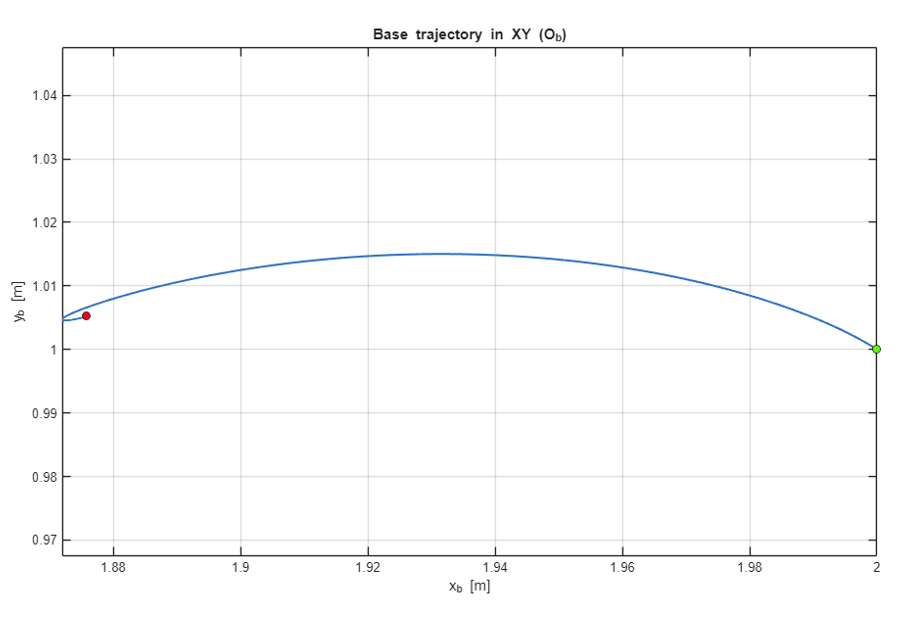
\includegraphics[width=\columnwidth]{figures/E1_layer1_only_base_path_world.png}
  \caption{Layer~1 only (dynamic feedback linearization): base motion in the
  world frame. Layer~1 enforces torque-level tracking but requires a
  task-consistent reference generated by higher layers.}
  \label{fig:E1_layer1_base}
\end{figure}

% ---------------------------------------------------------
\subsection{Planner Only: Offline Reference Generation (Open-Loop)}
\label{subsec:res_planner_only}
% ---------------------------------------------------------
We next evaluate the offline planner alone (open-loop), to verify that it
generates smooth, dynamically trackable references for both the base and the
arm. The base trajectory is produced in $\mathrm{SE}(2)$ using the
rotate--translate--rotate construction with quintic time-scaling, while the arm
joints are generated using quintic polynomials satisfying endpoint boundary
conditions.

Fig.~\ref{fig:E2_planner_base} shows the planned base path in the world frame.
Figs.~\ref{fig:E2_planner_eta}--\ref{fig:E2_planner_etaddot} confirm that the
planner produces smooth reference profiles in $\etav$, including continuous
velocity and acceleration. This smoothness is essential because the torque-level
controller uses $\etavddot_d$ (explicitly or implicitly) to shape the closed-loop
error dynamics; discontinuous or noisy references can induce large transient
torques and poor robustness.

\begin{figure}[t]
  \centering
  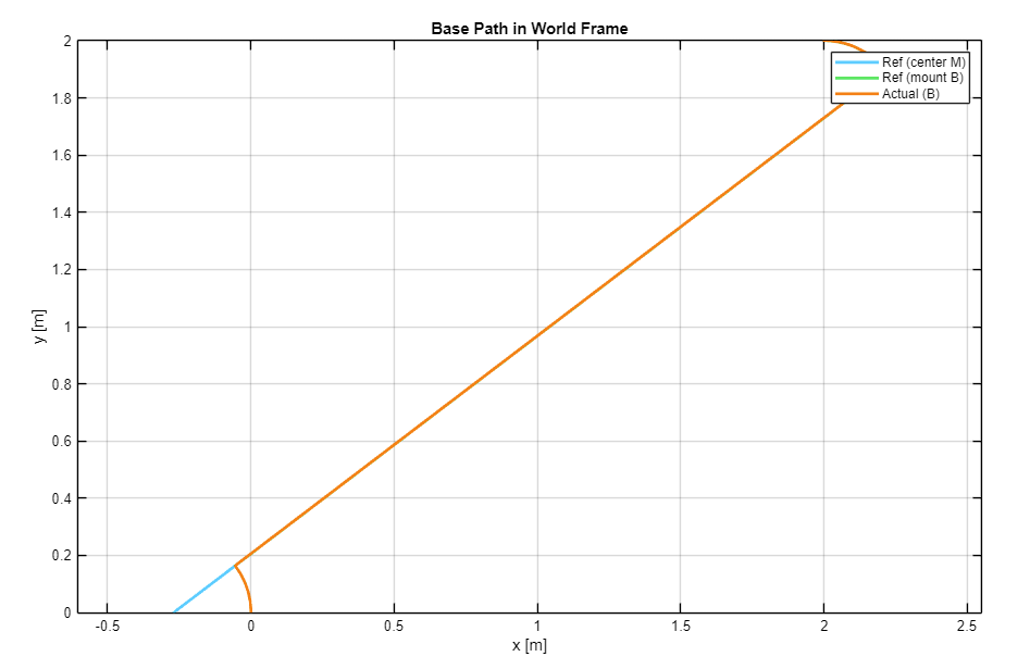
\includegraphics[width=\columnwidth]{figures/E2_planner_only_base_path_world.png}
  \caption{Planner-only (open-loop): planned base path in the world frame.}
  \label{fig:E2_planner_base}
\end{figure}

\begin{figure}[t]
  \centering
  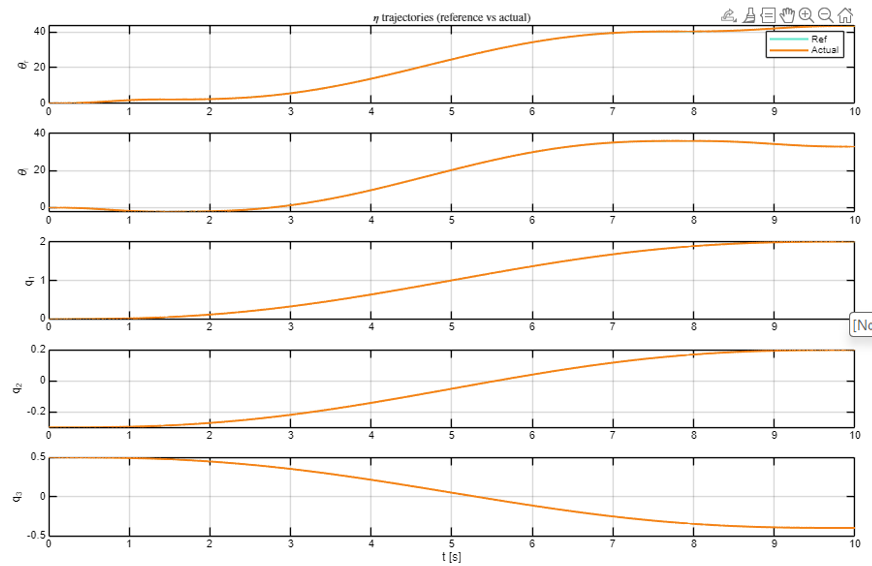
\includegraphics[width=\columnwidth]{figures/E2_planner_only_eta.png}
  \caption{Planner-only (open-loop): reference $\etav_d(t)$ (wheel angles and arm
  joint angles).}
  \label{fig:E2_planner_eta}
\end{figure}

\begin{figure}[t]
  \centering
  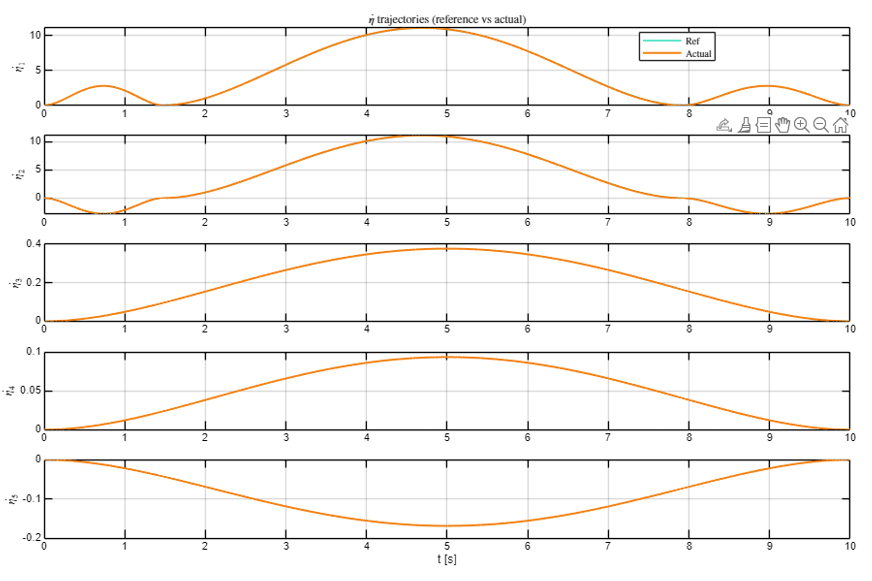
\includegraphics[width=\columnwidth]{figures/E2_planner_only_etadot.png}
  \caption{Planner-only (open-loop): reference $\etavdot_d(t)$.}
  \label{fig:E2_planner_etadot}
\end{figure}

\begin{figure}[t]
  \centering
  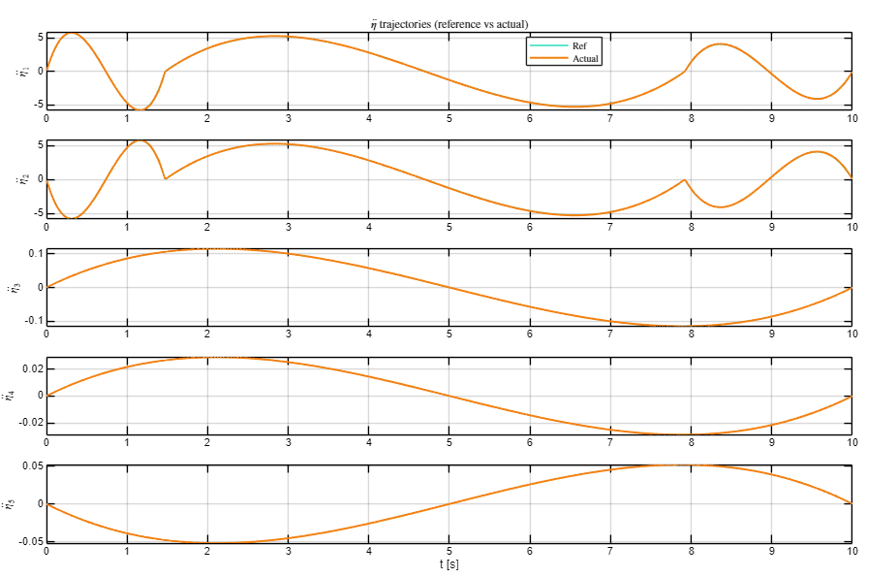
\includegraphics[width=\columnwidth]{figures/E2_planner_only_etaddot.png}
  \caption{Planner-only (open-loop): reference $\etavddot_d(t)$ (smooth
  acceleration profiles suitable for torque-level tracking).}
  \label{fig:E2_planner_etaddot}
\end{figure}

% ---------------------------------------------------------
\subsection{Disturbance Without Feedback Compensation}
\label{subsec:res_dist_no_feedback}
% ---------------------------------------------------------
To highlight the need for closed-loop coordination and feedback mechanisms under
uncertainty, we inject additive torque disturbances and evaluate performance
without the full inter-layer feedback support. Fig.~\ref{fig:E3_dist_base}
illustrates that disturbance causes visible deviation from the intended base
trajectory. The corresponding deviation in the reduced coordinates is shown in
Fig.~\ref{fig:E3_dist_eta}. These results motivate the use of the complete
three-layer architecture, where kinematic coordination and torque-level tracking
act together to reject disturbances and recover the desired motion.

\begin{figure}[t]
  \centering
  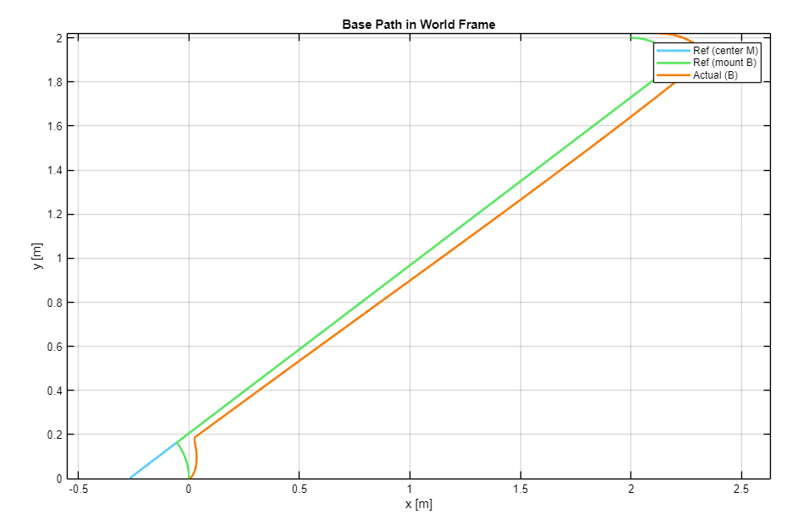
\includegraphics[width=\columnwidth]{figures/E3_dist_base_path_world.png}
  \caption{Under torque disturbance without full feedback compensation: base path
  deviates from the desired motion.}
  \label{fig:E3_dist_base}
\end{figure}

\begin{figure}[t]
  \centering
  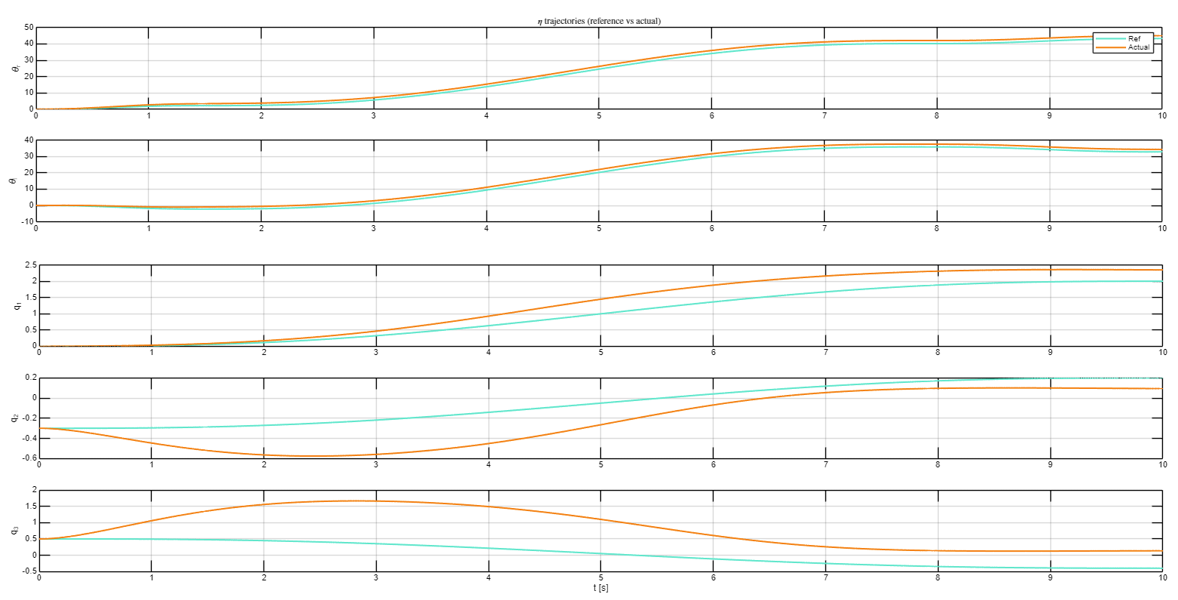
\includegraphics[width=\columnwidth]{figures/E3_dist_eta.png}
  \caption{Under torque disturbance without full feedback compensation:
  deviation in $\etav(t)$.}
  \label{fig:E3_dist_eta}
\end{figure}

% ---------------------------------------------------------
\subsection{Full Three-Layer Stack Under Disturbance}
\label{subsec:res_full_stack_dist}
% ---------------------------------------------------------
Finally, we activate the full three-layer stack and repeat the disturbance
experiment. The planner provides smooth offline references, the kinematic layer
generates admissible velocity commands for the base and arm, and the dynamic
layer applies feedback linearization to track the resulting reduced-coordinate
references at the torque level.

Fig.~\ref{fig:E4_dist_base} shows that the full stack preserves the desired base
motion despite disturbances. Figs.~\ref{fig:E4_dist_eta}--\ref{fig:E4_dist_etaddot}
show that reference tracking is maintained across $\etav$, $\etavdot$, and
$\etavddot$. The tracking error is summarized in
Fig.~\ref{fig:E4_dist_err_eta}, confirming convergence and bounded transient
response under disturbance.

To quantify control effort, Figs.~\ref{fig:E4_dist_tau_wheels} and
\ref{fig:E4_dist_tau_arm} report wheel and arm torques, respectively. The
instantaneous mechanical power $P(t)=\tau^\top(t)\etavdot(t)$ (watts) and the
accumulated control energy $E(t)=\int_0^t P(\sigma)\,d\sigma$ (joules) are shown
in Figs.~\ref{fig:E4_dist_power} and \ref{fig:E4_dist_energy}. These curves
enable a direct performance--effort comparison across conditions in a
reproducible manner.

\begin{figure}[t]
  \centering
  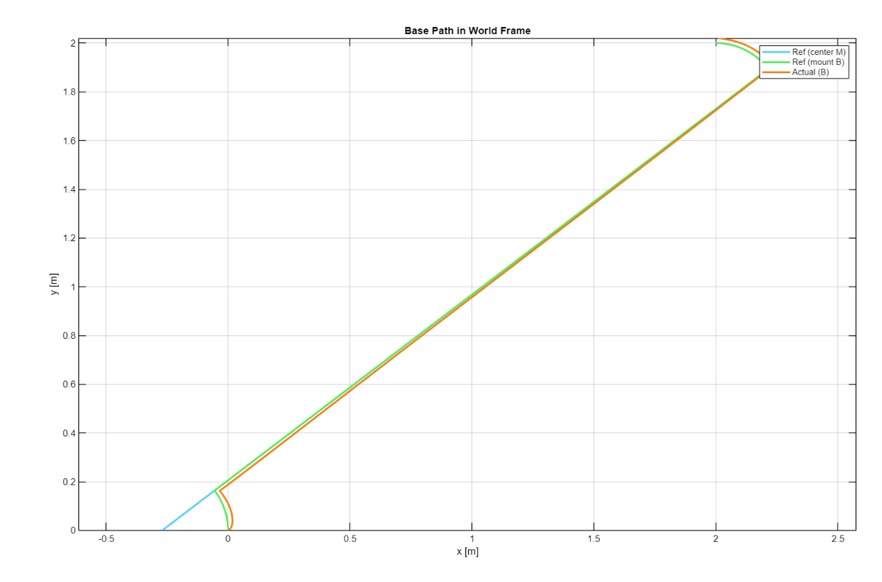
\includegraphics[width=\columnwidth]{figures/E4_dist_base_path_world.png}
  \caption{Full three-layer stack under torque disturbance: base path in the
  world frame remains close to the desired motion.}
  \label{fig:E4_dist_base}
\end{figure}

\begin{figure}[t]
  \centering
  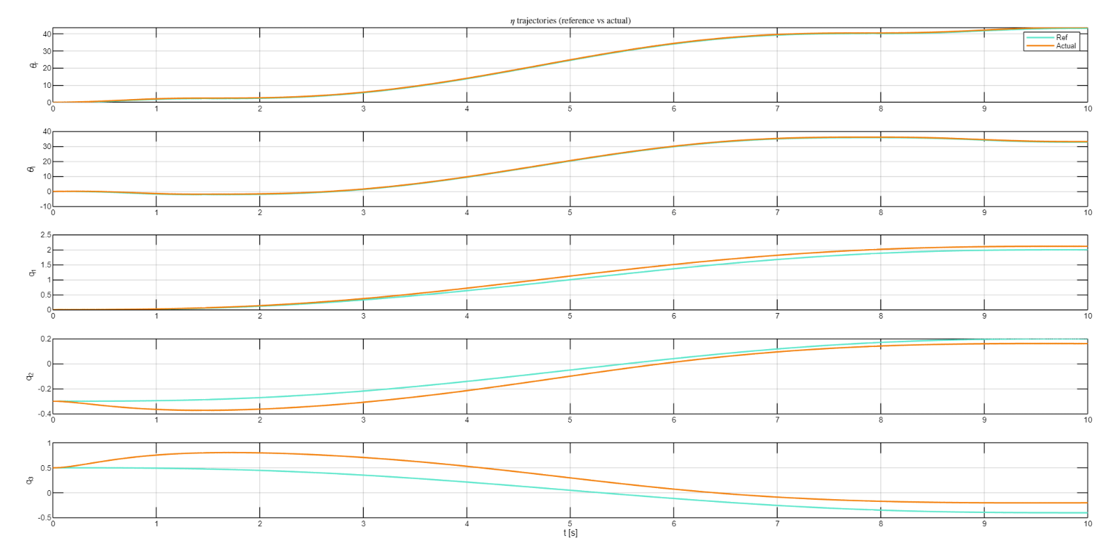
\includegraphics[width=\columnwidth]{figures/E4_dist_eta.png}
  \caption{Full stack under disturbance: tracking in $\etav(t)$.}
  \label{fig:E4_dist_eta}
\end{figure}

\begin{figure}[t]
  \centering
  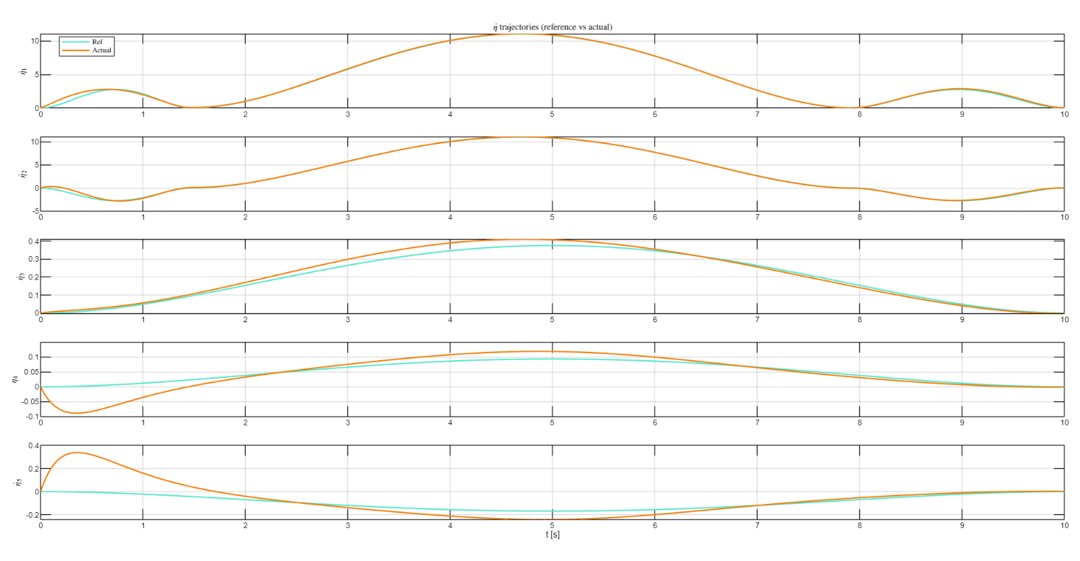
\includegraphics[width=\columnwidth]{figures/E4_dist_etadot.png}
  \caption{Full stack under disturbance: tracking in $\etavdot(t)$.}
  \label{fig:E4_dist_etadot}
\end{figure}

\begin{figure}[t]
  \centering
  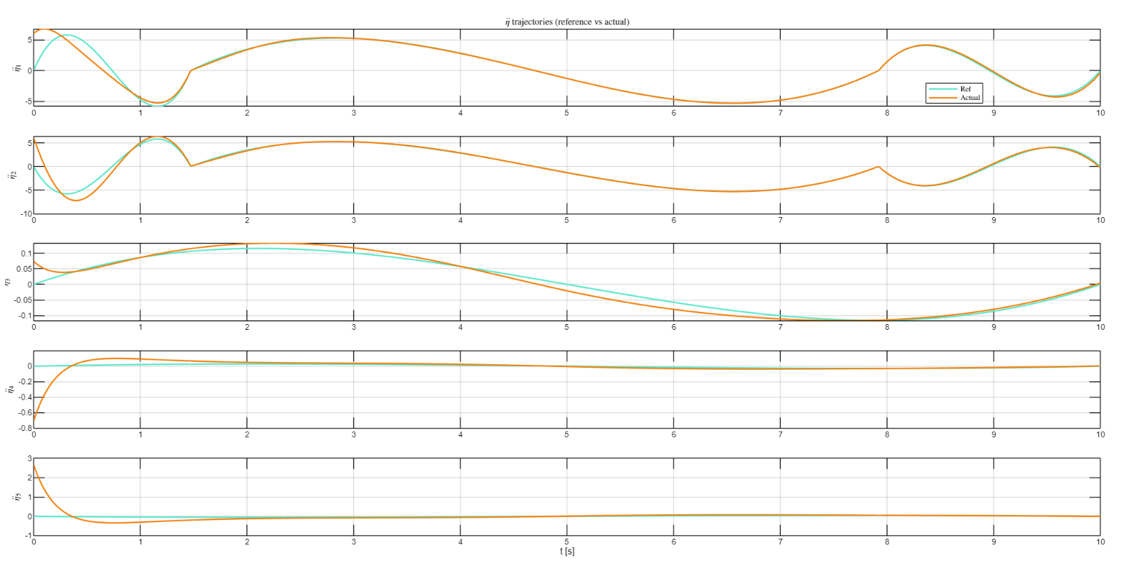
\includegraphics[width=\columnwidth]{figures/E4_dist_etaddot.png}
  \caption{Full stack under disturbance: tracking in $\etavddot(t)$.}
  \label{fig:E4_dist_etaddot}
\end{figure}

\begin{figure}[t]
  \centering
  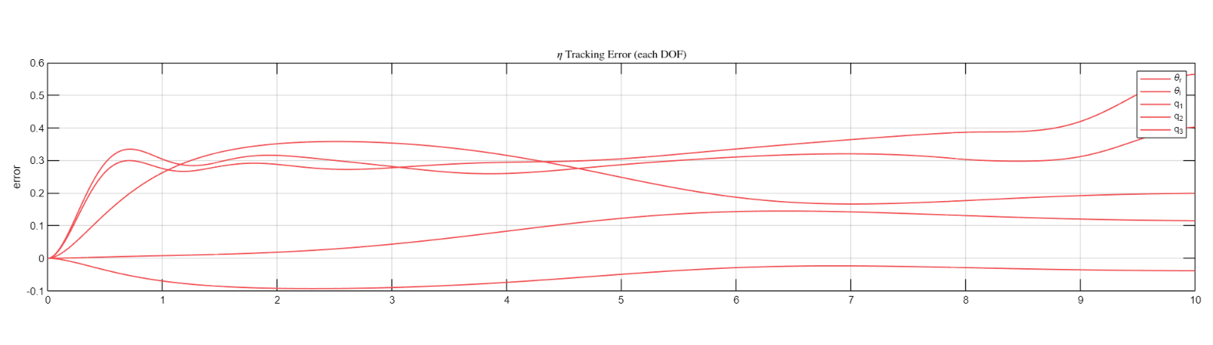
\includegraphics[width=\columnwidth]{figures/E4_dist_full_tracking_error_eta.png}
  \caption{Full stack under disturbance: tracking error in $\etav$ converges and
  remains bounded during disturbance transients.}
  \label{fig:E4_dist_err_eta}
\end{figure}

\begin{figure}[t]
  \centering
  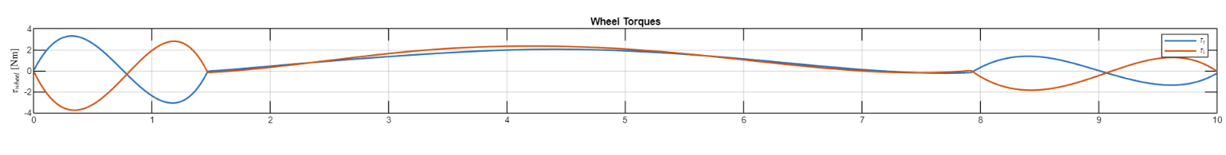
\includegraphics[width=\columnwidth]{figures/E4_dist_torque_wheels.png}
  \caption{Full stack under disturbance: wheel torques.}
  \label{fig:E4_dist_tau_wheels}
\end{figure}

\begin{figure}[t]
  \centering
  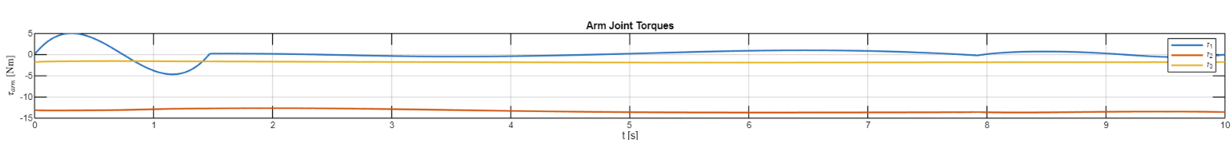
\includegraphics[width=\columnwidth]{figures/E4_dist_torque_arm.png}
  \caption{Full stack under disturbance: arm joint torques.}
  \label{fig:E4_dist_tau_arm}
\end{figure}

\begin{figure}[t]
  \centering
  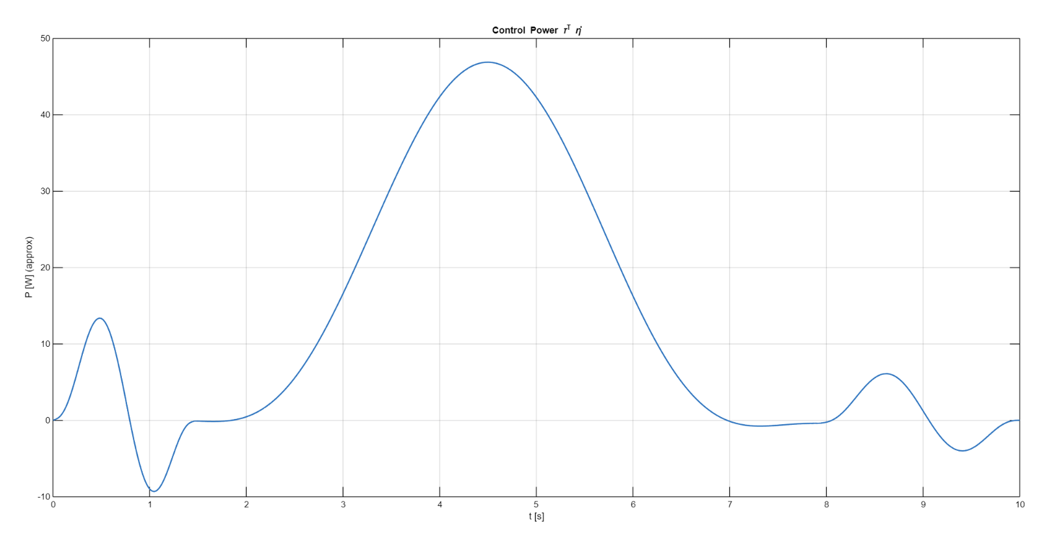
\includegraphics[width=\columnwidth]{figures/E4_dist_power.png}
  \caption{Full stack under disturbance: instantaneous mechanical power $P(t)$
  (watts).}
  \label{fig:E4_dist_power}
\end{figure}

\begin{figure}[t]
  \centering
  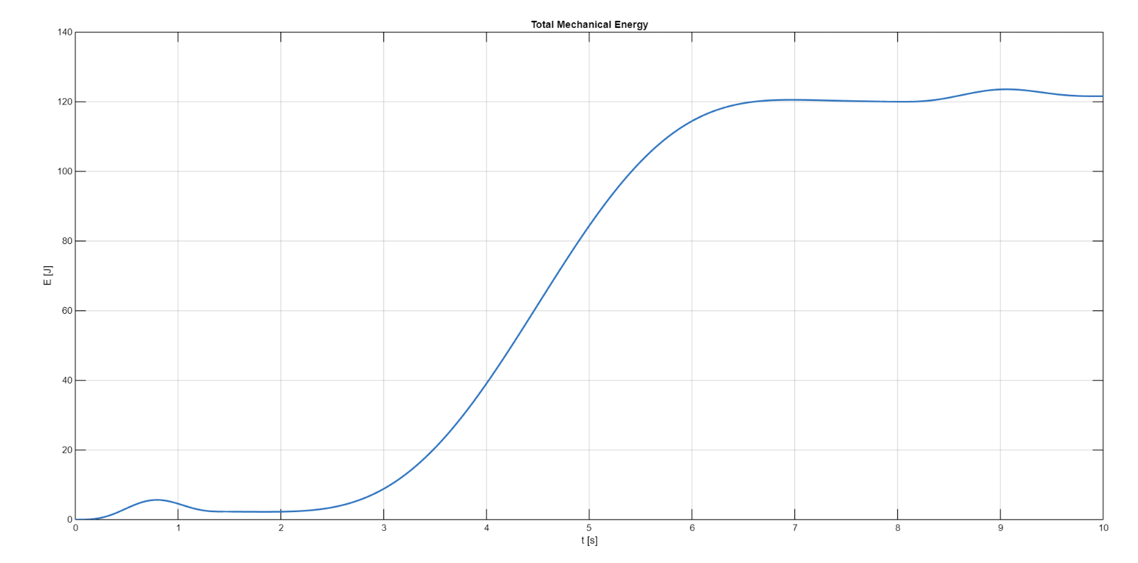
\includegraphics[width=\columnwidth]{figures/E4_dist_energy.png}
  \caption{Full stack under disturbance: accumulated control energy $E(t)$
  (joules).}
  \label{fig:E4_dist_energy}
\end{figure}

% ---------------------------------------------------------
\subsection{Summary of Key Findings}
\label{subsec:res_summary}
% ---------------------------------------------------------
The results support three main conclusions:
(i) Layer~1 provides accurate torque-level tracking but requires smooth,
task-consistent references from higher layers;
(ii) the offline planner generates $C^2$ references in $\etav$ that are suitable
for feedback linearization; and
(iii) under torque disturbances, the complete three-layer architecture maintains
trajectory tracking while providing interpretable effort metrics (torque, power,
and energy).


% =========================================================
\section{Discussion}
\label{sec:discussion}
% =========================================================
The presented results highlight why a differential-drive mobile manipulator
benefits from a layered design rather than relying on a single controller level.

\subsection{Why Layer~1 (Dynamics) Is Necessary but Not Sufficient}
Layer~1 (feedback linearization on the reduced coordinates $\etav$) provides a
clear advantage: it enforces second-order tracking error dynamics and directly
regulates torque inputs, which is essential when actuator effort, power, and
energy must be quantified and constrained. However, Layer~1 alone does not
define a task-consistent motion. In other words, it can track a given
$(\etav_d,\etavdot_d,\etavddot_d)$, but it cannot \emph{generate} these signals
from geometric objectives such as moving the base from $(x_0,y_0,\theta_0)$ to
$(x_f,y_f,\theta_f)$ while coordinating the arm motion. This explains why
planner-generated, smooth references are required in practice.

\subsection{Role of the Planner and Importance of Smooth References}
The offline planner produces time-parameterized trajectories that satisfy
boundary conditions and yield $C^2$ reference signals. This smoothness is not a
cosmetic feature: the torque-level tracker uses acceleration-level information
(either explicitly or through the structure of the tracking law), so reference
discontinuities can lead to impulse-like torques and degraded robustness.
Therefore, the planner is the mechanism that converts a task specification into
a dynamically trackable reference.

\subsection{Why a Kinematic Layer Is Needed Under Disturbances}
The disturbance experiments show that open-loop execution of the planned motion
can drift in the presence of torque disturbances and modeling mismatch. The
kinematic layer closes this gap by providing feedback at the velocity level,
regulating base and arm motion in task space and preventing geometric errors
(e.g., lateral and heading errors for the nonholonomic base) from accumulating.
When combined with Layer~1, the overall stack achieves both: (i) geometric
consistency at the motion level and (ii) disturbance rejection and effort-aware
tracking at the torque level.

\subsection{Energy and Effort Interpretation}
Power and accumulated energy plots provide an interpretable measure of control
effort beyond tracking error alone. Power captures instantaneous actuator demand
(watts), while accumulated energy (joules) summarizes the overall effort over
the task horizon. These metrics enable reproducible comparisons across
conditions (nominal vs.\ disturbed) and across tuning choices, and they are
directly relevant for actuator sizing and battery-budget reasoning.

\subsection{Limitations and Practical Considerations}
Several limitations should be noted. First, the current evaluation focuses on
simulation with a fixed scenario and offline planning; real systems will also
require state estimation, actuator saturation handling, and careful treatment of
unmodeled friction and delays. Second, gains were selected to yield
well-damped second-order error dynamics; more aggressive tuning may reduce
tracking error further but can increase torque peaks and energy consumption.
Finally, extending the planner to online replanning would improve adaptability
in dynamic environments, but introduces computational constraints and stability
questions that must be addressed.

% =========================================================
\section{Conclusion}
\label{sec:conclusion}
% =========================================================
This paper presented a unified planning and control framework for a
differential-drive mobile manipulator using a three-layer architecture:
(1) an offline $\mathrm{SE}(2)$ + joint-space planner that generates smooth
time-parameterized references, (2) a kinematic feedback layer that regulates
geometric tracking, and (3) a torque-level dynamic controller using feedback
linearization in reduced coordinates $\etav$ to impose second-order tracking
error dynamics.

Simulation results demonstrated that: (i) the dynamic controller alone can
achieve accurate torque-level tracking but requires task-consistent reference
generation; (ii) the planner provides smooth $C^2$ trajectories suitable for
dynamic tracking; and (iii) under injected torque disturbances, the full
three-layer stack maintains convergence and bounded tracking errors while
offering quantitative effort measures through torque, power, and accumulated
energy.

Future work will focus on (i) online replanning for changing goals and dynamic
obstacles, (ii) incorporation of actuator limits and friction models, and
(iii) experimental validation on hardware with state estimation and sensor
noise.

\bibliographystyle{IEEEtran}
\bibliography{mm_refs}

\end{document}
